\documentclass[]{hspf_thesis} 
\usepackage{lipsum}
\usepackage{tabularx}
\usepackage{times} % Needed to automatically update the date
\usepackage{soul}
\usepackage{xltabular}
% hyperref is already loaded in hspf_thesis.cls with [hidelinks]
\usepackage{enumitem} % <--- This is vital for the [leftmargin=*] part
\usepackage{ragged2e} % Wichtig für sauberen Umbruch in X-Spalten
\usepackage{booktabs} % Für schöne horizontale Linien
\usepackage{caption}
\usepackage{listings}
\usepackage{svg}
\usepackage{amsmath}
\usepackage[utf8]{inputenc}
\usepackage[babel=true,german=quotes]{csquotes}
\usepackage[table]{xcolor}

\usepackage{etoolbox}

% makeglossaries is already called in hspf_thesis.cls

\lstset{
  inputencoding=utf8,
  extendedchars=true,
  literate=
   {ä}{{\"a}}1
   {ö}{{\"o}}1
   {ü}{{\"u}}1
   {Ä}{{\"A}}1
   {Ö}{{\"O}}1
   {Ü}{{\"U}}1
   {ß}{{\ss}}1
}


% Zitation Einstellungen
\usepackage[backend=biber, style=ieee, citestyle=ieee]{biblatex}
\ExecuteBibliographyOptions{sorting=none}
\addbibresource{./bib/ProjektarbeitMovelink.bib}

% Institutionen
\newacronym{hspf}{HSPF}{Hochschule Pforzheim}

% Kernsystem
\newacronym{bde}{BDE}{Betriebsdatenerfassung}
\newacronym{eis}{EIS}{elektronische Informationssystem}
\newacronym{erp}{ERP}{Enterprise-Resource-Planning}

% Architektur- und Design-Prinzipien
\newacronym{adp}{ADP}{Acyclic Dependencies Principle}
\newacronym{srp}{SRP}{Single Responsibility Principle}
\newacronym{soc}{SoC}{Separation of Concerns}
\newacronym{ocp}{OCP}{Open/Closed Principle}
\newacronym{dry}{DRY}{Don't Repeat Yourself}


% Metriken
\newacronym{lcom}{LCOM}{Lack of Cohesion of Methods}
\newacronym{loc}{LOC}{Lines of Code}

% Methodik
\newacronym{moscow}{MoSCoW}{Must, Should, Could, Won't}

% Technologien und Protokolle
\newacronym{rest}{REST}{Representational State Transfer}
\newacronym{mqtt}{MQTT}{Message Queuing Telemetry Transport}
\newacronym{api}{API}{Application Programming Interface}
\newacronym{crud}{CRUD}{Create, Read, Update, Delete}
\newacronym{smtp}{SMTP}{Simple Mail Transfer Protocol}
\newacronym{json}{JSON}{JavaScript Object Notation}
\newacronym{mfc}{MFC}{Microsoft Foundation Classes}
\newacronym{sip}{SIP}{Session Initiation Protocol}
\newacronym{kmu}{KMU}{Kleine und mittlere Unternehmen}



\begin{document}
\begin{titlematter}
    \newgeometry{left=3.5cm,right=2.5cm,top=1.5cm,bottom=2.5cm}

\begin{titlepage}
    % Komplett serifenlose Schrift für das Deckblatt (wie in der Vorlage)
    % \sffamily 
    
    % Logo oben rechts
    \begin{flushright}
        
\includegraphics[width=0.4\textwidth]{img/HKALogo.png}
    \end{flushright}

    \vspace{2cm}
    
    \begin{flushleft}
        % Name und Matrikelnummer
        \large
        \textbf{Erlind Sejdiu} \\
        \textbf{106357}
        
        \vspace{4cm}
        
        % Titel der Arbeit
        \LARGE
        \textbf{Exposé: Evaluierung des nRF-Ökosystems und Zephyr RTOS für ressourcenbeschränkte IoT-Anwendungen anhand eines Wearable-Prototyps}
        
        \vspace{4cm}
        
        % Thesis Details
        \normalsize
        \textbf{Projektarbeit} \\
        \textbf{der Hochschule Karlsruhe} \\
        \textbf{im Master Studiengang Informatik} \\
        \textbf{im Sommersemester 2026}
        
        % Schiebt den Rest ganz nach unten an den Seitenrand
        \vfill 
        
        % Prüfer linksbündig ausgerichtet
        \normalsize
        \begin{tabular}{@{} l l }
            \textbf{Korrektor}: & Prof. Dr. rer. nat. Carsten Sinz \\
        \end{tabular}
        
    \end{flushleft}        
\end{titlepage}

\restoregeometry % Setzt die Ränder für das restliche Dokument wieder auf Standard zurück
\end{titlematter}
\begin{frontmatter}
    %\newgeometry{left=3.5cm,right=2.5cm,top=2.5cm,bottom=2cm}
\section*{Selbstständigkeitserklärung (ehrenwörtlichen Erklärung)}

\vspace{1cm}

Hiermit versichere ich, Erlind Sejdiu, die vorliegende Arbeit selbständig verfasst zu 
haben. Die aus fremden Quellen direkt oder indirekt übernommenen Texte, Gedankengänge, Konzepte, Grafiken usw. habe ich als solche gekennzeichnet und mit vollständigen Verweisen auf die jeweilige Quelle versehen. Weiter wurde die Arbeit bisher nicht an einer anderen Stelle zur Prüfung vorgelegt.

Ich habe Künstliche Intelligenz als Ausführungs- und Gestaltungswerkzeug eingesetzt, bin mir
jedoch bewusst, dass die Nutzung maschinell generierter Texte, Grafiken, Bilder, Bewegtbilder,
Codes etc. keine Garantie für Qualität und Korrektheit gewährleistet. Ich verantworte die Übernahme jeglicher von mir verwendeter maschinell generierter Passagen vollumfänglich selbst und trage Verantwortung, falls es zu fehlerhaften Inhalten, zu Verstößen gegen das Datenschutzrecht, das Urheberrecht oder zu wissenschaftlichem Fehlverhalten (z. B. Plagiate) kommt. Ich versichere, dass in der vorliegenden Arbeit mein intellektueller und gestalterischer Einfluss überwiegt und ich beim Einsatz KI-gestützter Werkzeuge steuernd gearbeitet habe. Ich habe keine KI-Tools verwendet, deren Nutzung der Prüfer/die Prüferin explizit schriftlich ausgeschlossen hat. Zusätzlich versichere ich, dass ich KI-gestützte Werkzeuge in der Rubrik „Übersicht verwendeter Hilfsmittel“ mit ihrem Produktnamen, meiner Bezugsquelle (z. B. URL) und Angaben zu genutzten Funktionen der Software sowie zum Nutzungsumfang vollständig aufgeführt habe. Weitere Vorgaben der Prüfer*innen zur Dokumentation habe ich entsprechend beachtet.

\paragraph{Sperrvermerk}
Die vorliegende Arbeit enthält firmeninterne Informationen und vertrauliche Daten der ProSeS BDE GmbH. Sie darf aus diesem Grunde nur zu Prüfzwecken verwendet und ohne ausdrückliche Genehmigung durch ProSeS BDE GmbH weder Dritten zugänglich gemacht noch ganz oder in Auszügen veröffentlicht werden.


\begin{comment}
\begin{figure}[H]
    
\includegraphics[width=0.3\textwidth,right=13cm]{img/Unterschrift.png}
\end{figure}
\end{comment}
\begin{figure}[h]
    \begin{minipage}{0.5\textwidth}
        \vspace{1cm}
        Pforzheim, 28.02.2026 \newline \newline 
        Ort, Datum
    \end{minipage}
    \begin{minipage}{0.5\textwidth}
        
\includegraphics[width=0.5\textwidth]{img/Unterschrift.png} \newline
        Unterschrift 
    \end{minipage}
\end{figure}

%\hspace{2cm} Ort, Datum \hfill Unterschrift \hspace{2cm}
    %\section*{Kurzfassung}
Das elektronische Informationssystem (EIS) der Firma ProSeS versendet automatisierte Benachrichtigungen über verschiedene Kanäle, wie SMS, E-Mail und eine Smartphone-App. Aufgrund der kontinuierlichen Erweiterung des bestehenden Systems ohne begleitende architektonische Anpassungen sind eine hohe Komponentenkopplung und eine eingeschränkte Wartbarkeit entstanden. Ziel dieser Arbeit war daher die Neuentwicklung des EIS.

In einem iterativen Erhebungsprozess wurden elf funktionale Anforderungen priorisiert und 13 nicht-funktionale Anforderungen auf Basis der Wartbarkeitsdefinition der ISO 25010 mit messbaren Abnahmekriterien festgelegt. Darauf aufbauend wurde eine Client-Server-Architektur entworfen. Das Angular-Frontend dient als Konfigurationsoberfläche zur Regelerstellung und -verwaltung. Das C\#-Backend verarbeitet eingehende Ereignisse und steuert den Versand. Für das Backend wurde eine hexagonale Architektur gewählt, die das Hinzufügen neuer Versandkanäle ermöglicht, ohne dass die bestehende Geschäftslogik verändert werden muss.

Die Evaluation zeigt, dass alle als Muss eingestuften funktionalen Anforderungen erfüllt wurden. Die Wartbarkeitsanalyse mittels statischer Analysewerkzeuge belegt im Vergleich zum Altsystem eine höhere Wartbarkeit anhand der ausgewählten Indikatoren. Insgesamt legen die Ergebnisse eine verbesserte strukturelle Grundlage für die langfristige Weiterentwicklung nahe.
    %\glsresetall
\newpage
\section*{Abstract} 
The electronic information system (EIS) from ProSeS sends automated notifications via various channels, such as SMS, email, and a smartphone app. Due to the continuous expansion of the existing system without accompanying architectural adjustments, a high degree of component coupling and limited maintainability have resulted. The aim of this work was therefore to redevelop the EIS.

In an iterative survey process, eleven functional requirements were prioritized and 13 non-functional requirements were defined based on the maintainability definition of ISO 25010 with measurable acceptance criteria. Based on this, a client-server architecture was designed. The Angular front end serves as a configuration interface for rule creation and management. The C\# backend processes incoming events and controls dispatch. A hexagonal architecture was chosen for the backend, which allows new dispatch channels to be added without having to change the existing business logic.

The evaluation shows that all functional requirements classified as mandatory have been met. The maintainability analysis using static analysis tools confirms higher maintainability compared to the legacy system based on the selected indicators. Overall, the results suggest an improved structural basis for long-term further development.
    \glsaddall
    %\newpage
    \inhaltsverzeichnis
\end{frontmatter}

\begin{mainmatter}

    %\section{Einleitung}
%\label{ch:Einleitung}

\section{Motivation}
Durch die fortschreitende Vernetzung im Rahmen des Internet of Things (IoT) werden intelligente, eingebettete Systeme zunehmend Teil unseres Alltags. Selbst kleinste Alltagsgegenstände sind heutzutage in der Lage, mit ihrem Umfeld zu kommunizieren und Daten zu erfassen. Typische Beispiele hierfür sind Smart-Home-Komponenten sowie Smart-Wearables wie smarte Gesundheitsringe. So entwickelt die Firma DIO beispielsweise Ringe, die Parameter wie Puls und Bewegungsgeschwindigkeit messen können \cite{noauthor_smart_nodate}. Parallel dazu durchdringt die Vernetzung auch den privaten Wohnraum immer stärker. Smart-Home-Geräte erfassen kontinuierlich Umgebungsdaten, wie etwa die Luftqualität, und übermitteln diese zur Auswertung an mobile Endgeräte \cite{noauthor_smart_nodate-1}.

In vielen dieser kompakten Smart-Devices haben sich die nRF-System-on-Chips (SoCs) von Nordic Semiconductor etabliert, da sie hinsichtlich Energieeffizienz, Baugröße und Funktionalität gängige Industriestandards erfüllen. Die Kehrseite dieser leistungsfähigen Hardware ist jedoch ein hochkomplexes Software-Ökosystem. Für moderne nRF-Chips wird offiziell die Nutzung des Echtzeitbetriebssystems Zephyr RTOS in Verbindung mit dem nRF Connect SDK empfohlen. Diese Toolchain führt jedoch abstrakte Konzepte wie DeviceTrees und Kconfig ein, deren Beherrschung eine steile Lernkurve erfordert \cite{noauthor_nordic_2023, noauthor_25_nodate}.

\section{Problemstellung}
\label{sec:Aufgabenstellung}
Das zentrale Problem, das in dieser Arbeit adressiert wird, ist die hohe Software-Komplexität des Zephyr RTOS bei der Programmierung moderner System-on-Chips (SoCs). Obwohl Zephyr zunehmend als Industriestandard empfohlen wird, gilt die Entwicklung als überaus anspruchsvoll, da spezifische Architekturkonzepte wie DeviceTrees und Kconfig ein tiefgehendes Systemverständnis voraussetzen \cite{noauthor_25_nodate}.

Um diese Komplexität greifbar zu machen, erfolgt die Untersuchung methodisch anhand der iterativen Entwicklung eines funktionsfähigen Prototyps. Dieser praktische Anwendungsfall soll systematisch veranschaulichen, welcher Entwicklungsaufwand tatsächlich erforderlich ist, um grundlegende Funktionalitäten innerhalb dieses Ökosystems erfolgreich bereitzustellen.

Zur klaren Abgrenzung der Problemstellung: Der Fokus der Arbeit liegt ausschließlich auf der Embedded-Softwareentwicklung und der Architektur, nicht auf dem Hardware- oder PCB-Design. Ebenso ist es nicht das Ziel, mithilfe des Prototyps valide medizinische oder industrielle Testdaten zu erheben. Das Hauptaugenmerk liegt vielmehr auf der softwareseitigen Evaluierung und der Komplexität, die zur Implementierung der jeweiligen Features bewältigt werden muss.

\section{Stand der Technik}
\label{sec:Stand der Technik}
In der aktuellen Literatur finden sich bereits diverse Vergleiche von Betriebssystemen für das Internet of Things und für eingebettete Systeme. Zumeist liegt der Fokus dabei jedoch auf allgemeinen Architekturkonzepten oder reinen Leistungsmessungen, während die praktische Entwicklerperspektive weitgehend unberücksichtigt bleibt.

Ein Beispiel für einen solchen theoretischen Vergleich liefert die Arbeit von Kanwal et al. \cite{kanwal_iot_2023}. Die Autoren evaluieren verschiedene IoT-Betriebssysteme anhand ihrer Architektur, Programmiermodelle, Scheduling-Verfahren und Speicherverwaltung. Diese Analyse verbleibt jedoch auf einer rein konzeptionellen Ebene und trifft keine verlässliche Aussage darüber, wie aufwendig sich die praktische Konfiguration und Implementierung in den jeweiligen Systemen gestaltet.

Andere Arbeiten dringen zwar tiefer in die Praxis ein und testen Systeme wie Zephyr, RIOT und Contiki-NG auf ressourcenbeschränkter Hardware, jedoch beschränken sich auch diese Benchmarks primär auf die reine Netzwerkleistung. Der tatsächliche Entwicklungsaufwand für die Schaffung dieser Programmfunktionalitäten wird nicht bewertet \cite{silva_operating_2019}.

Neben wissenschaftlichen Publikationen existieren zahlreiche praxisnahe Artikel aus der Industrie (sogenannte graue Literatur), wie beispielsweise der Beitrag \textit{„Measuring Real-Time Operating System Performance Part II: Comparing FreeRTOS vs. Zephyr“} \cite{noauthor_measuring_nodate}. Derartige Analysen konzentrieren sich oft eng auf hardwarenahe Laufzeitmetriken wie Taktzyklen, Interrupt-Latenzen oder die Dauer eines Context-Switches.

Zusammenfassend lässt sich festhalten, dass der aktuelle Stand der Technik vorrangig die Hardware-Performance oder die theoretische Architektur der Betriebssysteme beleuchtet. Was jedoch weitreichend fehlt, ist eine detaillierte Analyse der \textit{Komplexität der Software-Entwicklung}. Es wird kaum untersucht, wie hoch der Overhead und die Einstiegshürden für Entwickler tatsächlich sind, wenn sie sich – wie bei Zephyr unvermeidlich – in abstrakte Konfigurationssprachen wie \texttt{Kconfig} und \texttt{DeviceTrees} einarbeiten müssen. 

Die vorliegende Arbeit zielt darauf ab, genau diese Forschungslücke zu schließen: Anstatt lediglich zu messen, wie schnell und effizient der finale Code auf dem Mikrocontroller ausgeführt wird, soll systematisch erarbeitet werden, welcher praktische Aufwand erforderlich ist, um grundlegende Funktionalitäten innerhalb des Zephyr-Ökosystems initial bereitzustellen.

\section{Forschungsfrage}
\label{sec:Forschungsfrage}
Aus der beschriebenen Problemstellung sowie dem aktuellen Stand der Technik leitet sich folgende zentrale Forschungsfrage ab:

\textit{Wie verhält sich der Overhead des Zephyr RTOS – insbesondere hinsichtlich des Konfigurationsaufwands sowie des Flash- und RAM-Bedarfs – zur tatsächlichen Applikations-Nutzlast bei einer einfachen Sensor-Edge-Anwendung?}

Zur Beantwortung dieser Frage werden die konkreten Stärken, Schwächen und technischen Herausforderungen analysiert, die während der Implementierungsphase auftreten. Das übergeordnete Ziel dieser Projektarbeit besteht somit in einer systematischen und praxisnahen Evaluation der nRF-Technologie und des Zephyr-Ökosystems anhand der Entwicklung eines iterativen Prototyps.

\section{Methodik}
Um die Forschungsfrage fundiert zu beantworten, wird im Rahmen dieser Projektarbeit ein funktionsfähiger Prototyp für ein verteiltes IoT-Sensornetzwerk im Bereich der Bewegungsanalyse entwickelt.

In diesem Anwendungsszenario interagieren mehrere IoT-Geräte miteinander, um die Bewegungen menschlicher Körperteile anhand von Beschleunigungs- und Gyroskopdaten zu erfassen. Perspektivisch ließen sich diese Daten nutzen, um Bewegungsabläufe zu bewerten – etwa zur Überprüfung der korrekten Ausführung physiotherapeutischer Übungen. Wie bereits erläutert, verbleibt der Fokus hierbei jedoch strikt auf der Evaluierung von Zephyr als Plattform für verteilte Systeme und nicht auf der Gewinnung medizinisch verwertbarer Kennzahlen.

Das methodische Vorgehen umfasst die Konzeption und Entwicklung eines Systems, das insgesamt aus drei Geräten besteht: zwei Sensor-Knoten zur Datenerfassung sowie einem zentralen Endgerät (z.\,B. einem Smartphone oder PC) für den Datenempfang (siehe \autoref{fig:System Aufbau von Movelink}).

\begin{figure}[H]
    \centering
    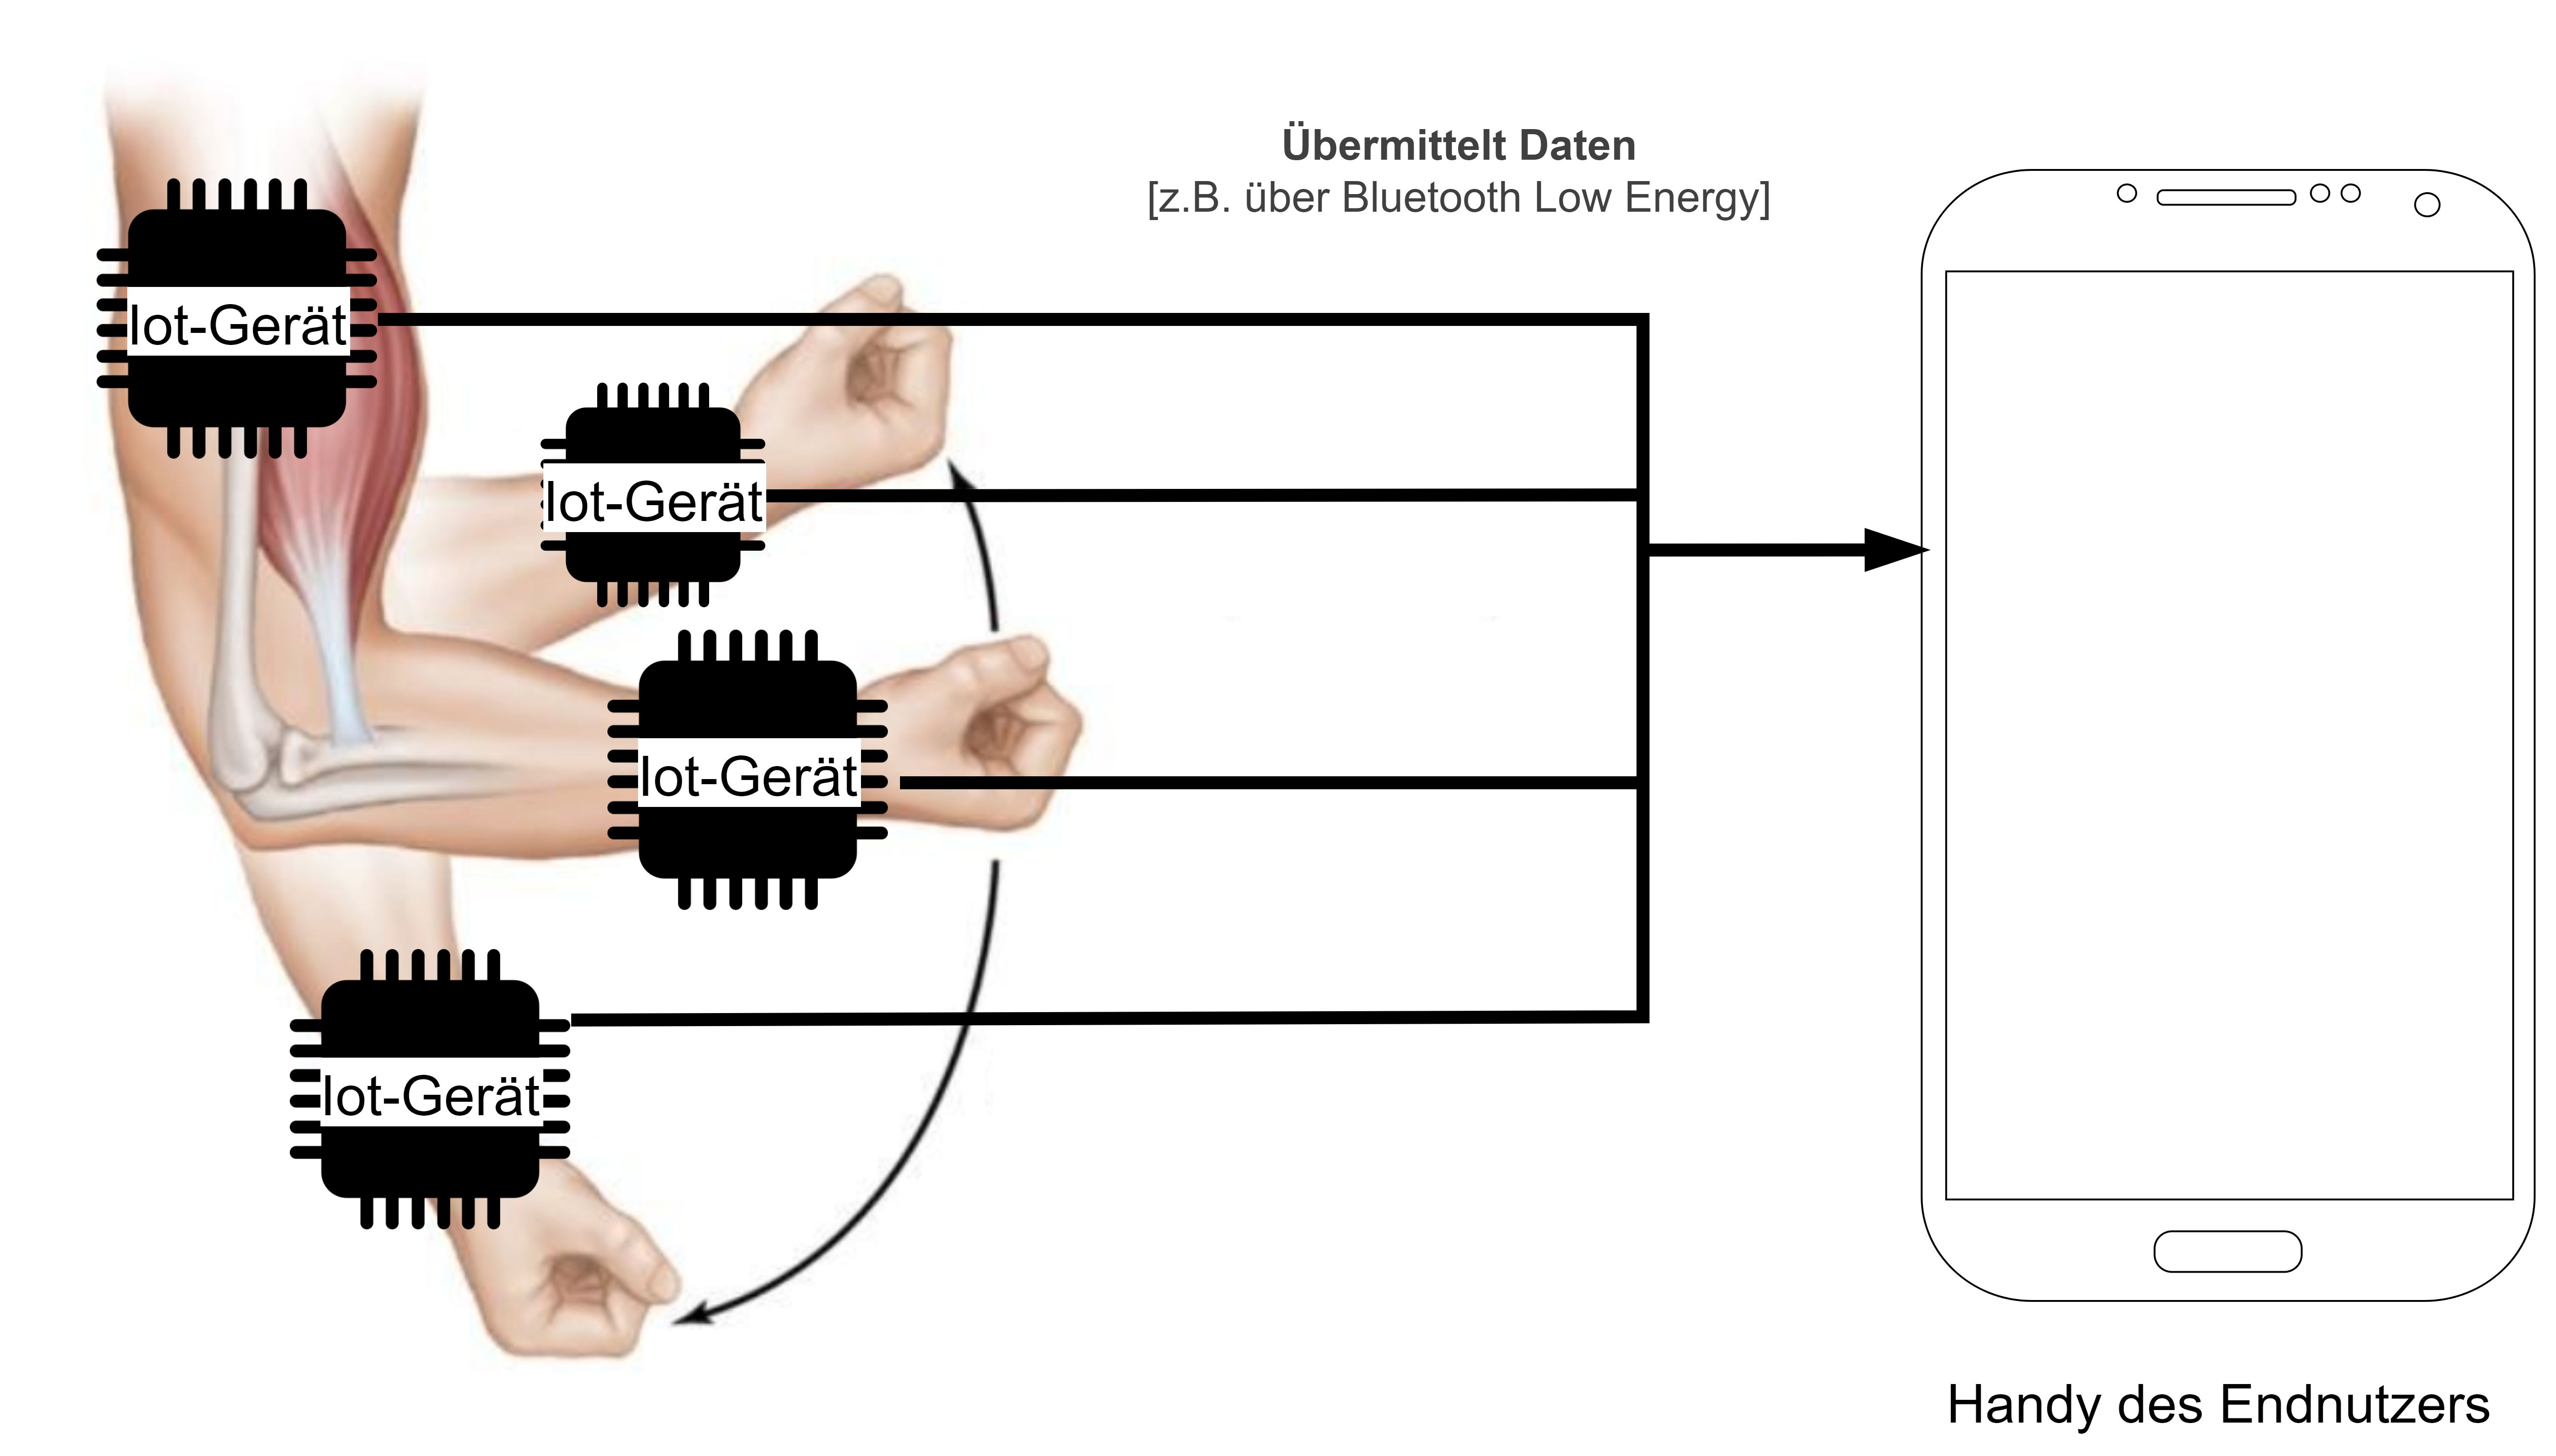
\includegraphics[width=0.9\linewidth]{img/SchematischeDarstellung.png}
    \caption{Abstrakter Software-Aufbau}
    \label{fig:System Aufbau von Movelink}
\end{figure}


Um den Entwicklungsaufwand quantifizierbar zu machen, wird der Prototyp schrittweise aufgebaut und soll vier Kernfunktionalitäten abbilden:

\begin{itemize}
    \item \textbf{„Hello World“ (Blinkende LED \& Button-Interrupt):} \\ Ziel ist die Schaffung einer funktionalen Baseline zur Validierung der grundlegenden Toolchain.
    \item \textbf{Sensorintegration (z.\,B. I2C-Kommunikation mit einem IMU-Sensor):} \\ Ziel ist das Testen der hardwarenahen Peripherie-Anbindung sowie das zyklische Auslesen der Sensordaten.
    \item \textbf{1-to-1-Konnektivität (Datenübertragung an eine Gegenstelle):} \\ Ziel ist die Implementierung einer direkten drahtlosen Kommunikation zwischen zwei Knoten.
    \item \textbf{1-to-N-Konnektivität (Datenübertragung im Netzwerk):} \\ Ziel ist die Erweiterung des Aufbaus zu einem Sensornetzwerk mit mehreren interagierenden Geräten.
\end{itemize}

Bei jedem dieser Meilensteine wird erfasst, in welchem Verhältnis der Code-Overhead (Konfigurationsdateien, Setup) zum eigentlichen Applikationscode steht. Parallel dazu wird dokumentiert, wie sich der RAM- und Flash-Speicherbedarf mit jeder neuen Funktionsebene vergrößert. Diese gesteigerte Systemkomplexität liefert fundierte Erhebungswerte zur Beantwortung der Forschungsfrage.

Eine detaillierte Auflistung der funktionalen und nicht-funktionalen Systemanforderungen befindet sich dem Dokumentenanhang.

\section{Zeitplan}

Um einen strukturierten Projektfortschritt zu gewährleisten, wurden den einzelnen Entwicklungsphasen konkrete Ziele und Artefakte zugeordnet. Diese Meilensteine bilden das Fundament der Evaluierung:

\begin{description}
    \item[Phase 1: Vorbereitung und Setup] \hfill \\
    \textbf{Ziel:} Schaffung der infrastrukturellen Basis für die praktische Implementierung sowie grundlegende Einarbeitung in die Konzepte von Zephyr und nRF Connect. \\
    \textbf{Artefakt:} Eine vollständig konfigurierte Toolchain (nRF Connect SDK) sowie ein einfaches „Hello World“-Basisprojekt, das lauffähig auf das Zielsystem (XIAO nRF52840 Sense) geflasht wurde.
    
    \item[Phase 2: Prototyping Basis (Hardware \& Sensorik)] \hfill \\
    \textbf{Ziel:} Erfolgreiche Ansteuerung der Hardware-Peripherie und einfache Verarbeitung der I2C-Sensordaten. \\
    \textbf{Artefakt:} Eine Firmware, die über den DeviceTree korrekt auf den integrierten IMU-Sensor zugreift, die Rohdaten des Beschleunigungs- und Gyroskopsensors ausliest, filtert und seriell (UART/RTT) ausgibt.
    
    \item[Phase 3: Kommunikation] \hfill \\
    \textbf{Ziel:} Etablierung einer drahtlosen, echtzeitfähigen Kommunikationsschnittstelle auf Basis von Bluetooth Low Energy (BLE). \\
    \textbf{Artefakt:} Eine Firmware-Erweiterung, die die formatierten Sensordaten drahtlos an ein Smartphone (etwa über die nRF Connect Mobile-App) sowie zweitweise an einen weiteren Empfänger-Mikrocontroller streamt.
    
    \item[Phase 4: Evaluation (Technischer Abschluss)] \hfill \\
    \textbf{Ziel:} Datenerhebung zur kritischen Betrachtung der Forschungsfrage bezüglich der Vor- und Nachteile des nRF/Zephyr-Stacks. \\
    \textbf{Artefakt:} Ein detailliertes Mess- und Evaluationsprotokoll, das sowohl quantitative Metriken (etwa Flash-/RAM-Bedarf, Code-Ratio) als auch eine qualitative Dokumentation der aufgetretenen Barrieren (besonders DeviceTree und Kconfig) umfasst.
    
    \item[Phase 5: Ausarbeitung] \hfill \\
    \textbf{Ziel:} Wissenschaftliche Aufbereitung, Diskussion und schriftliche Reflexion der gesammelten Projekterkenntnisse. \\
    \textbf{Artefakt:} Die finale schriftliche Dokumentation der Projektarbeit inklusive dokumentiertem Quellcode (versioniert in einem Git-Repository).
\end{description}

\begin{figure}[H]
    \centering
    % We change \textwidth to \textheight here so it stretches from top to bottom
    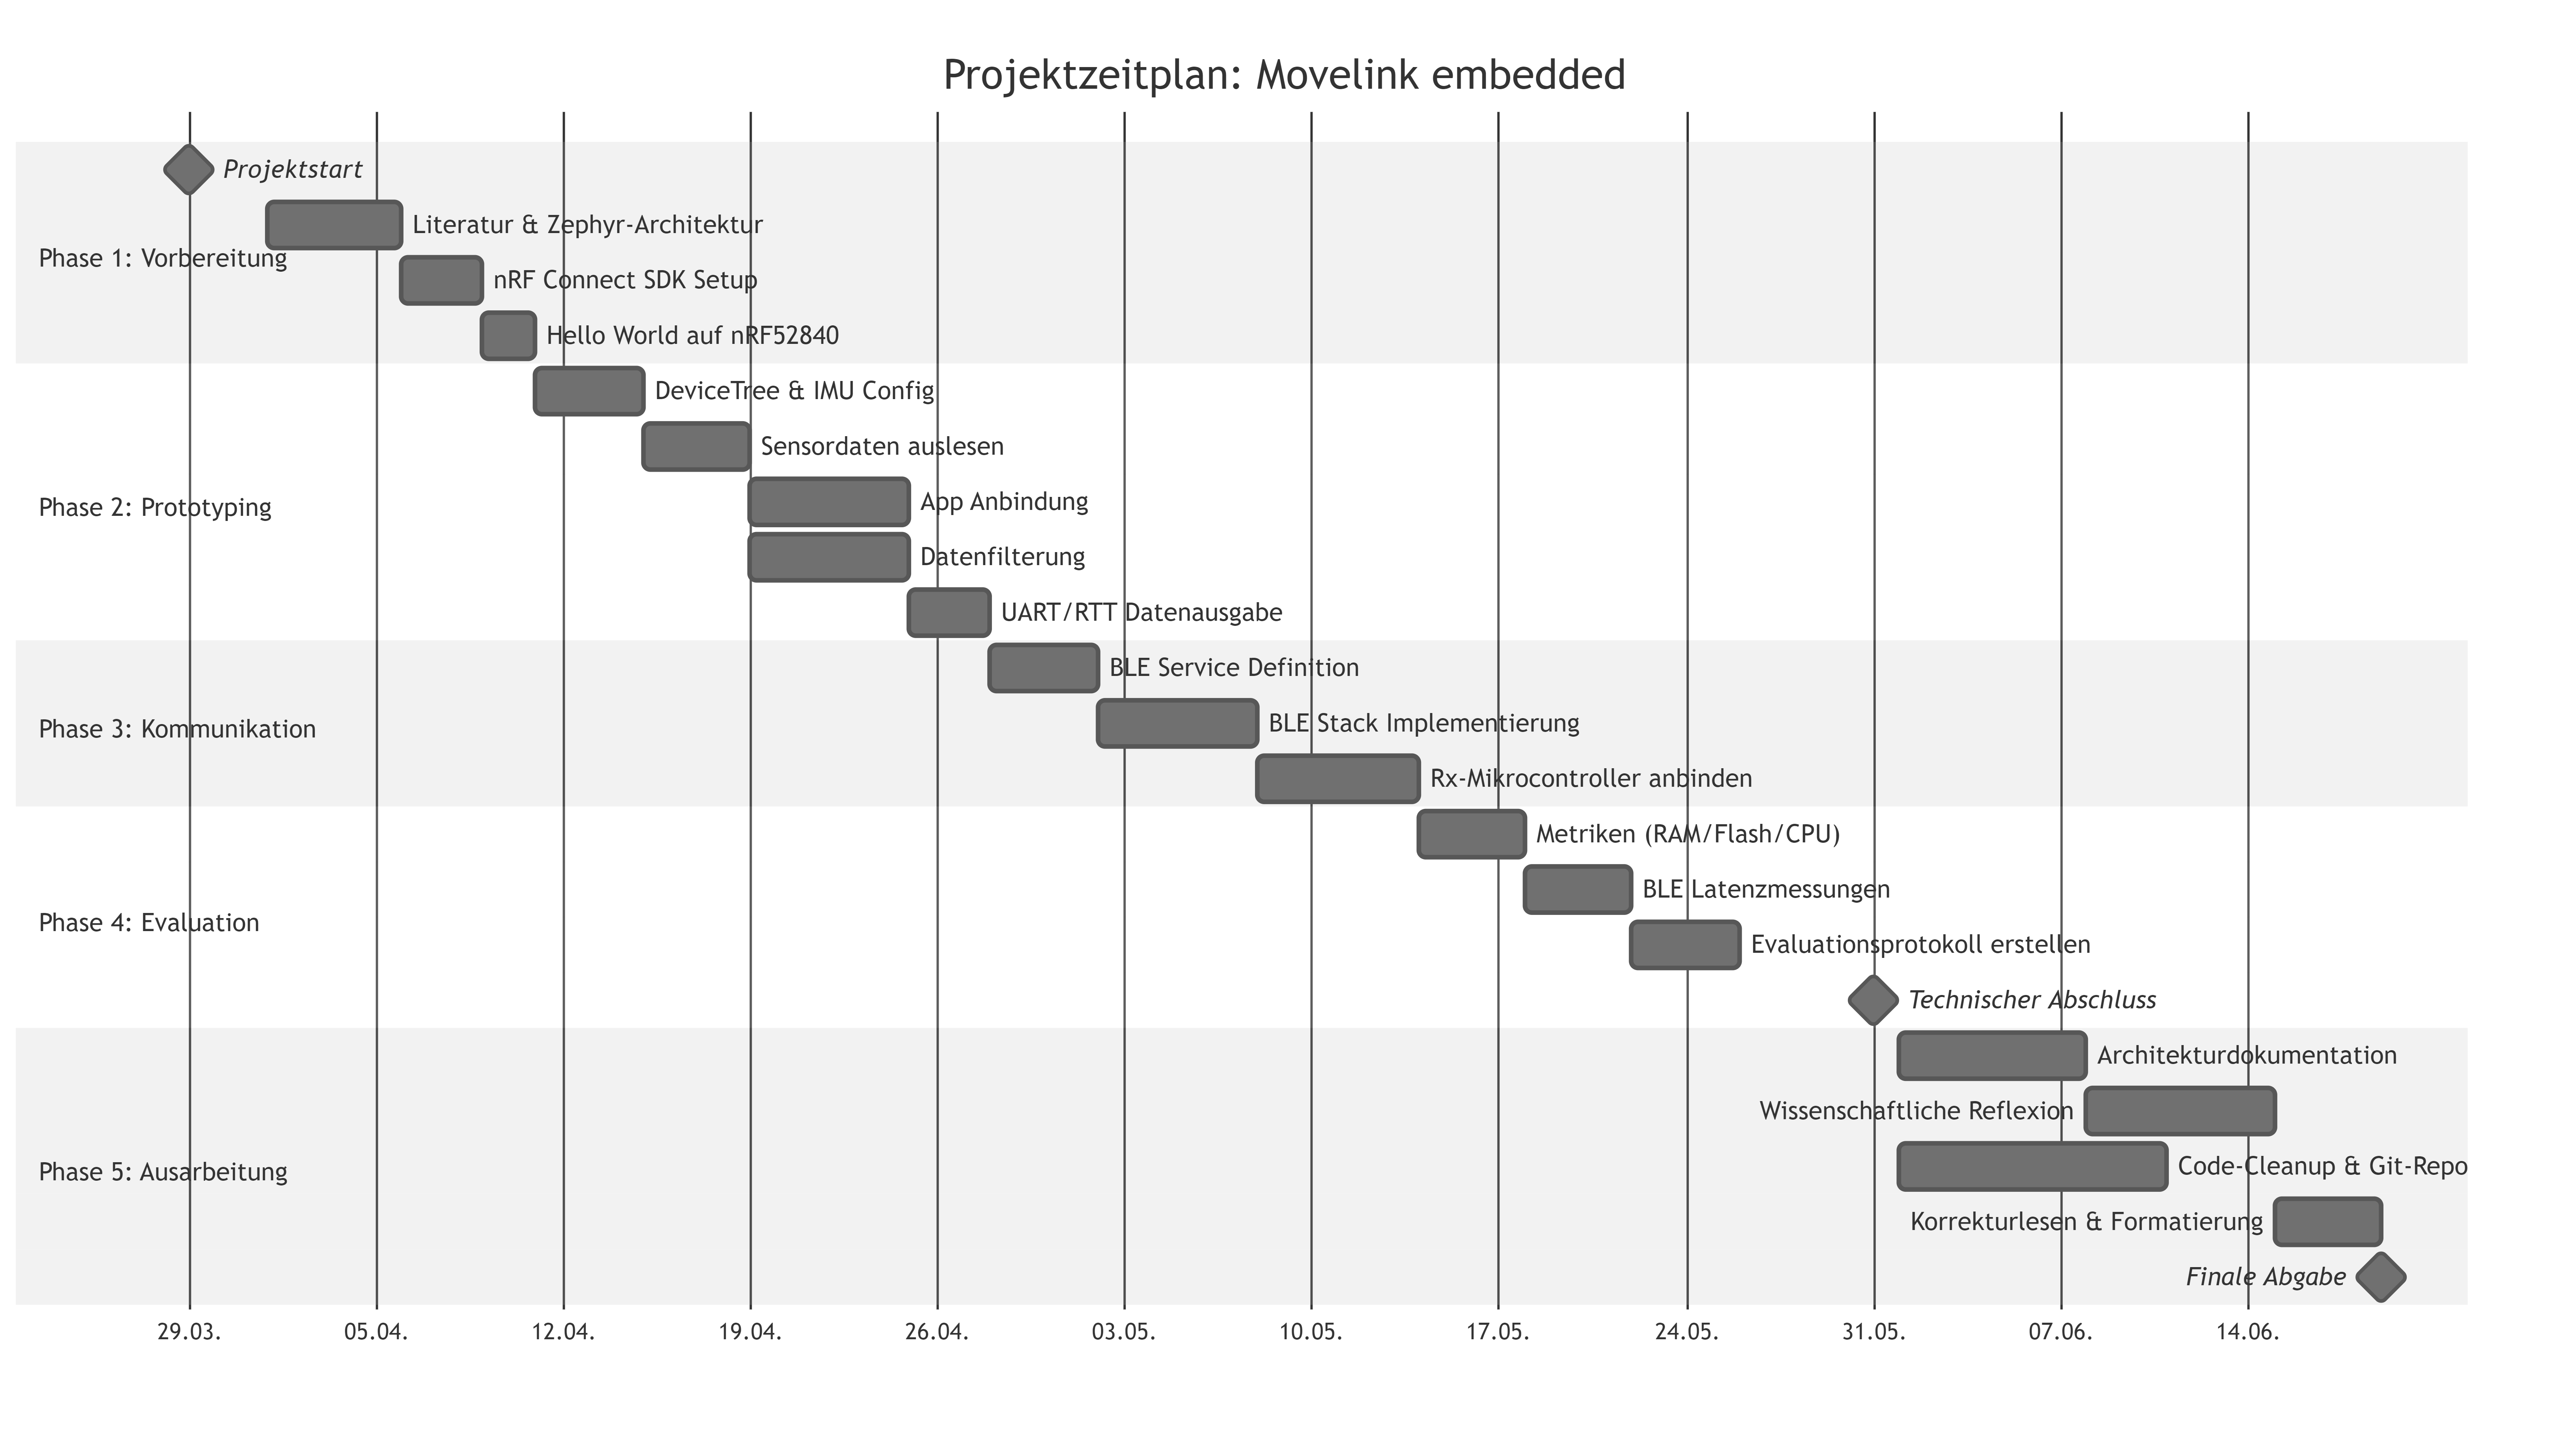
\includegraphics[angle=90, height=0.95\textheight, width=0.95\textwidth, keepaspectratio]{img/zeitplan.png}
    \caption{Zeitplan: Movelink embedded}
    \label{fig:zeitplan}
\end{figure}
    %\section{Stand der Technik}
\label{sec:StandDerTechnik}

Gegenwärtige Forschungsarbeiten und Publikationen evaluieren Betriebssysteme für eingebettete Systeme und das Internet of Things (IoT) vorrangig anhand architektonischer Eigenschaften sowie ihrer Ausführungsleistung. 

Eine umfassende qualitative Analyse verschiedener IoT-Betriebssysteme liefern \textit{Kanwal et al. (2023)}\footnote{\url{https://www.mdpi.com/2079-9292/12/3/708}}. Sie vergleichen unterschiedliche Betriebssysteme hinsichtlich Kernkriterien wie OS-Architektur, Programmiermodellen, Scheduling, Speicherverwaltung, Dateisystemen, sowie spezifischen Vor- und Nachteilen (Advantages und Limitations). Dabei bleibt die Betrachtung jedoch primär auf einer summarischen und konzeptionellen Ebene, ohne eine tiefergehende quantitative Bewertung der Implementierungs- und Konfigurationskomplexität vorzunehmen.

Darüber hinaus existieren Studien wie jene von \textit{Silva et al. (2019)}\footnote{\url{https://ieeexplore.ieee.org/document/8835860}}, die Contiki-NG, RIOT und Zephyr explizit auf ressourcenbeschränkten Geräten (Low-End Devices) vergleichen. Während hier ausführliche operative Benchmarks durchgeführt werden, liegt der Fokus in der Auswertung hauptsächlich auf der Verarbeitungszeit innerhalb des Netzwerkverkehrs und dem Verhalten der Betriebssysteme unter verschiedenen Lastbedingungen (Network Stack Benchmarks).

Zusätzlich finden sich in der technischen Praxis und industrienahen Publikationen (Grey Literature) Berichte, die spezifische Low-Level-Laufzeiteigenschaften vergleichen. Ein repräsentatives Beispiel hierfür ist die Publikation \textit{„Measuring Real-Time Operating System Performance Part II: Comparing FreeRTOS vs. Zephyr“}\footnote{\url{https://interrupt.memfault.com/blog/rtos-performance-freertos-vs-zephyr-part-2}}. Solche Analysen widmen sich den zeitlichen Verhaltensweisen von Echtzeitbetriebssystemen und vergleichen Metriken wie benötigte Taktzyklen, Interrupt-Latenzen oder Context-Switch-Zeiten. Eine ganzheitliche Gegenüberstellung, die den Entwicklungsaufwand, die Toolchain-Komplexität (beispielsweise durch Konzepte wie \texttt{Kconfig} und \texttt{DeviceTree} im Zephyr-Ökosystem) oder den Konfigurations-Overhead berücksichtigt, findet nicht statt.

\subsection{Zusammenfassung und Abgrenzung}
Zusammenfassend lässt sich feststellen, dass der aktuelle Stand der Technik Betriebssysteme zumeist detailliert miteinander vergleicht – sei es auf konzeptioneller Ebene oder durch Leistungsmessungen direkt auf dem Edge-Device. Eine pragmatische Analyse, die bewertet, wie hoch die initiale \textit{Komplexität} bei der konkreten Firmware-Erstellung ist, fehlt jedoch. Oftmals werden lediglich die reinen Taktzyklen und Latenzen einzelner Funktionen betrachtet, aber eine Analyse zur Verhältnismäßigkeit zwischen dem notwendigen Konfigurationsaufwand und der tatsächlichen Nutzlast (Features) steht noch aus. Genau hier setzt die vorliegende Arbeit an.

    %\section{Anforderungsanalyse}
\label{ch:Anforderungsanalyse}


    %\section{Konzeption der Softwarearchitektur}
\label{ch:Softwarearchitektur}

    %\section{Technische Umsetzung}
\label{ch:Implementierung}

    %
\clearpage
\section{Evaluation und Bewertung}
\label{ch:Evaluation}
\markboth{6 Evaluation und Bewertung}{}

    %
\section{Zusammenfassung und Ausblick}
\label{ch:Zusammenfassung}


    \appendix
    %\include{00_Vorderseiten/zeitplan}
    \literaturverzeichnis

    
    %\section{Nicht-funktionale Query-Metriken}
\renewcommand{\arraystretch}{1.5}
% Verkleinerte Schriftart für die gesamte Tabelle
\footnotesize
\begin{longtable}{|>{\raggedright\arraybackslash}p{0.13\textwidth}|>{\raggedright\arraybackslash}p{0.41\textwidth}|>{\raggedright\arraybackslash}p{0.41\textwidth}|}
\hline
\textbf{Metrik} & \textbf{C\# Query} & \textbf{C++ Query} \\ \hline
\endfirsthead

\multicolumn{3}{c}{{\bfseries \tablename\ \thetable{} -- Fortsetzung}} \\
\hline
\textbf{Metrik} & \textbf{C\# Query} & \textbf{C++ Query} \\ \hline
\endhead

\hline \multicolumn{3}{|r|}{{Fortsetzung auf der nächsten Seite...}} \\ \hline
\endfoot

\hline
\endlastfoot

NF1: Zyklom. Komplexität &
{\ttfamily
(from m in Application.Namespaces\newline
\quad .WithName(\newline
\quad \quad "ProBDE\_API\_Server.EIS")\newline
\quad .ChildMethods()\newline
where m.CyclomaticComplexity\newline
\quad .HasValue\newline
select (double)m.Cyclomatic\newline
\quad Complexity.Value).Average()
}
&
{\ttfamily
(from m in JustMyCode.Methods\newline
where m.CyclomaticComplexity\newline
\quad .HasValue\newline
select (double)m.Cyclomatic\newline
\quad Complexity.Value).Average()
}
\\ \hline

NF2: Doku-Grad &
{\ttfamily
(from m in Application.Namespaces\newline
\quad .WithName(\newline
\quad \quad "ProBDE\_API\_Server.EIS")\newline
\quad .ChildMethods()\newline
where m.PercentageComment\newline
\quad .HasValue\newline
select (double)m.Percentage\newline
\quad Comment.Value).Average()
}
&
{\ttfamily
(from m in JustMyCode.Methods\newline
where m.PercentageComment\newline
\quad .HasValue\newline
select (double)m.Percentage\newline
\quad Comment.Value).Average()
}
\\ \hline

NF3: LOC Gesamt &
{\ttfamily
Application.Namespaces\newline
\quad .WithName(\newline
\quad \quad "ProBDE\_API\_Server.EIS")\newline
\quad .ChildTypes()\newline
\quad .Where(t => t.NbLinesOfCode\newline
\quad \quad .HasValue)\newline
\quad .Sum(t => t.NbLinesOfCode.Value)
}
&
{\ttfamily
JustMyCode.Types\newline
\quad .Where(t => t.NbLinesOfCode\newline
\quad \quad .HasValue)\newline
\quad .Sum(t => t.NbLinesOfCode.Value)
}
\\ \hline

NF4: Verschach-telung &
{\ttfamily
(from m in Application.Namespaces\newline
\quad .WithName(\newline
\quad \quad "ProBDE\_API\_Server.EIS")\newline
\quad .ChildMethods()\newline
select (double)m.NestingDepth)\newline
\quad .Average()
}
&
{\ttfamily
(from m in JustMyCode.Methods\newline
select (double)m.NestingDepth)\newline
\quad .Average()
}
\\ \hline

NF5: Struktur. Rauschen &
{\ttfamily
(from m in Application.Namespaces\newline
\quad .WithName(\newline
\quad \quad "ProBDE\_API\_Server.EIS")\newline
\quad .ChildMethods()\newline
where m.CyclomaticComplexity\newline
\quad .HasValue \newline
\quad \&\& m.NbLinesOfCode.HasValue\newline
\quad \&\& m.CyclomaticComplexity\newline
\quad \quad .Value > 0 \newline
\quad \&\& m.NbLinesOfCode.Value > 0\newline
let ratio = (double)m.NbLinesOfCode\newline
\quad .Value / (double)m\newline
\quad .CyclomaticComplexity.Value\newline
select ratio).Average()
}
&
{\ttfamily
(from m in JustMyCode.Methods\newline
where m.CyclomaticComplexity\newline
\quad .HasValue \newline
\quad \&\& m.NbLinesOfCode.HasValue\newline
\quad \&\& m.CyclomaticComplexity\newline
\quad \quad .Value > 0 \newline
\quad \&\& m.NbLinesOfCode.Value > 0\newline
let ratio = (double)m.NbLinesOfCode\newline
\quad .Value / (double)m\newline
\quad .CyclomaticComplexity.Value\newline
select ratio).Average()
}
\\ \hline

NF6: Kohäsion (LCOM) &
{\ttfamily
from t in Application.Namespaces\newline
\quad .WithName(\newline
\quad \quad "ProBDE\_API\_Server.EIS")\newline
\quad .ChildTypes()\newline
where t.LCOM.HasValue \newline
\quad \&\& t.LCOM.Value > 0.8\newline
\quad \&\& t.NbMethods > 5 \newline
\quad \&\& t.NbFields > 3\newline
orderby t.LCOM.Value descending\newline
select new \{ t, \newline
\quad LCOM = t.LCOM.Value, \newline
\quad t.NbMethods, t.NbFields \}
}
&
{\ttfamily
warnif count > 0\newline
from t in JustMyCode.Types\newline
where t.LCOM.HasValue \newline
\quad \&\& t.LCOM.Value > 0.8\newline
\quad \&\& t.NbMethods > 5 \newline
\quad \&\& t.NbFields > 3\newline
orderby t.LCOM.Value descending\newline
select new \{ t, \newline
\quad LCOM = t.LCOM.Value, \newline
\quad t.NbMethods, t.NbFields \}
}
\\ \hline

NF7: API Kapselung &
{\ttfamily
from m in Application.Namespaces\newline
\quad .WithName(\newline
\quad \quad "ProBDE\_API\_Server.EIS")\newline
\quad .ChildMethods()\newline
where m.IsPublic\newline
\quad \&\& m.MethodsCallingMe.Any()\newline
\quad \&\& m.MethodsCallingMe\newline
\quad \quad .All(caller => caller.ParentType \newline
\quad \quad == m.ParentType)\newline
select new \{ m, m.Visibility, \newline
\quad Callers = m.MethodsCallingMe \}
}
&
{\ttfamily
from m in JustMyCode.Methods\newline
where m.IsPublic\newline
\quad \&\& m.MethodsCallingMe.Any()\newline
\quad \&\& m.MethodsCallingMe\newline
\quad \quad .All(caller => caller.ParentType \newline
\quad \quad == m.ParentType)\newline
select new \{ m, m.Visibility, \newline
\quad Callers = m.MethodsCallingMe \}
}
\\ \hline

NF8: Größen-Ausreißer &
{\ttfamily
from t in Application.Namespaces\newline
\quad .WithName(\newline
\quad \quad "ProBDE\_API\_Server.EIS")\newline
\quad .ChildTypes()\newline
where t.NbLinesOfCode.HasValue \newline
\quad \&\& t.NbLinesOfCode.Value > 200 \newline
\quad \&\& t.NbFields > 20\newline
orderby t.NbLinesOfCode.Value \newline
\quad descending\newline
select new \{ t, \newline
\quad LOC = t.NbLinesOfCode.Value, \newline
\quad t.NbMethods, t.NbFields \}
}
&
{\ttfamily
warnif count > 0\newline
from t in JustMyCode.Types\newline
where t.NbLinesOfCode.HasValue \newline
\quad \&\& t.NbLinesOfCode.Value > 200 \newline
\quad \&\& t.NbFields > 20\newline
orderby t.NbLinesOfCode.Value \newline
\quad descending\newline
select new \{ t, \newline
\quad LOC = t.NbLinesOfCode.Value, \newline
\quad t.NbMethods, t.NbFields \}
}
\\ \hline

NF9: Methoden-anzahl &
{\ttfamily
from t in Application.Namespaces\newline
\quad .WithName(\newline
\quad \quad "ProBDE\_API\_Server.EIS")\newline
\quad .ChildTypes()\newline
where t.NbMethods > 20\newline
orderby t.NbMethods descending\newline
select new \{ t, t.NbMethods, \newline
\quad LCOM = t.LCOM \}
}
&
{\ttfamily
warnif count > 0\newline
from t in JustMyCode.Types\newline
where t.NbMethods > 20\newline
orderby t.NbMethods descending\newline
select new \{ t, t.NbMethods, \newline
\quad LCOM = t.LCOM \}
}
\\ \hline

NF10: Ca-Risiko &
{\ttfamily
from t in Application.Namespaces\newline
\quad .WithName(\newline
\quad \quad "ProBDE\_API\_Server.EIS")\newline
\quad .ChildTypes()\newline
where t.NbTypesUsingMe > 50\newline
orderby t.NbTypesUsingMe descending\newline
select new \{ t, \newline
\quad IncomingDependencies = \newline
\quad \quad t.NbTypesUsingMe, \newline
\quad AbhaengigeKlassen = \newline
\quad \quad t.TypesUsingMe \}
}
&
{\ttfamily
warnif count > 0\newline
from t in JustMyCode.Types\newline
where t.NbTypesUsingMe > 50\newline
orderby t.NbTypesUsingMe descending\newline
select new \{ t, \newline
\quad IncomingDependencies = \newline
\quad \quad t.NbTypesUsingMe, \newline
\quad AbhaengigeKlassen = \newline
\quad \quad t.TypesUsingMe \}
}
\\ \hline

NF11: Zyklen &
{\ttfamily
from t in Application.Namespaces\newline
\quad .WithName(\newline
\quad \quad "ProBDE\_API\_Server.EIS")\newline
\quad .ChildTypes()\newline
where t.Level == null\newline
select new \{ t, \newline
\quad Status = "Zyklus erkannt", \newline
\quad t.NbTypesUsed, \newline
\quad t.NbTypesUsingMe \}
}
&
{\ttfamily
warnif count > 0\newline
from t in JustMyCode.Types\newline
where t.Level == null\newline
select new \{ t, \newline
\quad Warning = "Zyklus erkannt", \newline
\quad t.NbTypesUsed, \newline
\quad t.NbTypesUsingMe \}
}
\\ \hline

NF12: Kopplung &
{\ttfamily
from n in Application.Namespaces\newline
\quad .Where(x => x.Name == \newline
\quad \quad "ProBDE\_API\_Server.EIS")\newline
let types = n.ChildTypes\newline
\quad .Where(t => t.NbLinesOfCode > 0)\newline
let N = types.Count()\newline
let R = (from t in types\newline
\quad from usedType in t.TypesUsed\newline
\quad where usedType.ParentNamespace \newline
\quad \quad == n\newline
\quad select usedType).Count()\newline
let H = N > 0 ? \newline
\quad (double)(R + 1) / (double)N : 0\newline
select new \{ n, \newline
\quad RelationalCohesion = H, \newline
\quad AnzahlTypen = N, \newline
\quad InterneBeziehungen = R \}
}
&
{\ttfamily
warnif count > 0\newline
from n in Namespaces\newline
let types = n.ChildTypes\newline
\quad .Where(t => t.NbLinesOfCode > 0)\newline
let N = types.Count()\newline
let R = (from t in types\newline
\quad from usedType in t.TypesUsed\newline
\quad where usedType.ParentNamespace \newline
\quad \quad == n\newline
\quad select usedType).Count()\newline
let H = N > 0 ? \newline
\quad (double)(R + 1) / (double)N : 0\newline
where N > 3 \&\& \newline
\quad (H < 1.5 || H > 4.0)\newline
orderby H ascending\newline
select new \{ n, \newline
\quad RelationalCohesion = H, \newline
\quad AnzahlTypen = N, \newline
\quad InterneBeziehungen = R, \newline
\quad Warning = H < 1.5 ? \newline
\quad \quad "Zu schwach..." : "Zu komplex..." \}
}
\\ \hline

NF13: Duplikate &
{\ttfamily
from issue in ImportedIssues\newline
where issue.ToolName == "CPD" \newline
\quad \&\& issue.Type != null \newline
\quad \&\& issue.Type.ParentNamespace\newline
\quad \quad .Name == \newline
\quad \quad "ProBDE\_API\_Server.EIS"\newline
select new \{ issue, \newline
\quad Info = "Code-Duplikat im \newline
\quad \quad EIS Namespace" \}
}
&
{\ttfamily
warnif count > 0\newline
from issue in ImportedIssues\newline
where issue.ToolName == "CPD"\newline
select new \{ issue, \newline
\quad Warning = "Code-Duplikat \newline
\quad \quad entdeckt" \}
}
\\ \hline

\end{longtable}
\normalsize % Zurück zur normalen Größe
    %\newpage
    %\abbildungsverzeichnis
    %\tabellenverzeichnis
    %
\section*{Hilfsmittel}
\addcontentsline{toc}{section}{Hilfsmittel}
Übersicht verwendeter Hilfsmittel

\begin{enumerate}
    \item ChatGPT (GPT-5): Unterstützung bei sprachlichen Formulierungen, Recherche
und methodischer Ideenfindung. Keine inhaltliche Generierung wissenschaftlicher
Ergebnisse (https://chatgpt.com/)
    \item M365 Copilot: Unterstützung bei sprachlichen Formulierungen, Recherche und
methodischer Ideenfindung. Keine inhaltliche Generierung wissenschaftlicher Ergebnisse (https://m365.cloud.microsoft/chat)
    \item Google Gemini pro: Unterstützung bei sprachlichen Formulierungen, Recherche
und methodischer Ideenfindung. Keine inhaltliche Generierung wissenschaftlicher
Ergebnisse (https://gemini.google.com/app)
    \item DeepL Write: Formulierungs- und Rechtschreibhilfe für sprachlich anspruchsvolle
Teile der Arbeit zur Verbesserung der Lesbarkeit (https://www.deepl.com/de/write)
\end{enumerate}
    %\acronyme
    %\glossar
    



\end{mainmatter}


\end{document}